\documentclass[aspectratio=169]{beamer}
\usepackage{color,amsmath}
\usepackage{subfigure}
\usepackage{booktabs}
\usepackage{framed}
\usepackage{comment}
\usepackage{url}


%%%%%%%%%%%%%%%%%%%%%%%%%%
\title[]{Introduction to open-sourcing data}
\author[]{Matthew J. Salganik\\Department of Sociology\\Princeton University}
\date[]{Summer Institute in Computational Social Science\\June 21, 2018
\vfill
\begin{flushleft}
{\scriptsize
The Summer Institute in Computational Social Science is supported by grants from the Russell Sage Foundation and the Alfred P. Sloan Foundation.}
\end{flushleft}
\begin{flushright}

\includegraphics[width=0.1\textwidth]{figures/cc-by.png}
\end{flushright}
}
\begin{document}
%%%%%%%%%%%%%%%%%%%%%%%%%%
\frame{\titlepage}
%%%%%%%%%%%%%%%%%%%%%%%%%%
\begin{frame}

\begin{figure}
  \centering
  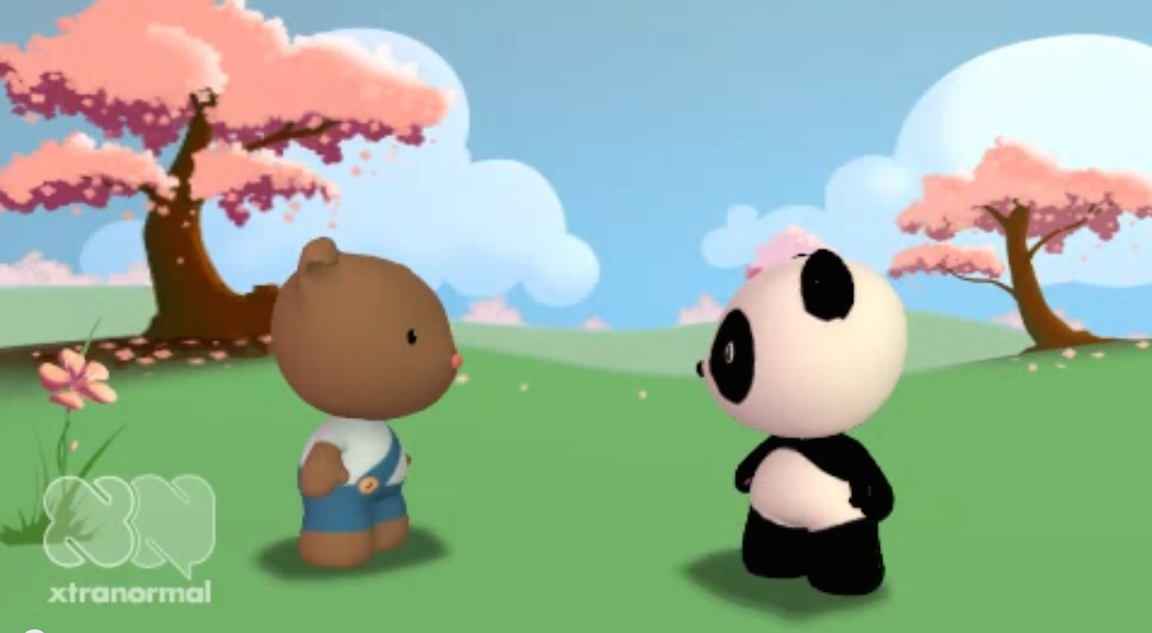
\includegraphics[width=0.9\textwidth]{figures/pandas_video}
\end{figure}

\url{https://www.youtube.com/watch?v=66oNv_DJuPc}

\end{frame}
%%%%%%%%%%%%%%%%%%%%%%%%%%%%%%%%
\begin{frame}

Brief introduction into open-sourcing your data:
\begin{itemize}
\item Store your data in a simple format
\pause
\item Provide documentation
\pause
\item Beware of privacy
\end{itemize}

\end{frame}
%%%%%%%%%%%%%%%%%%%%%%%%%%
\begin{frame}
\frametitle{Store your data in a simple format}

\pause
In this case .csv should be good.

\end{frame}
%%%%%%%%%%%%%%%%%%%%%%%%%%%
\begin{frame}
\frametitle{Provide documentation}

\pause
What would another researcher want to know? 

\begin{itemize}
\item How and when was this data collected?
\item What do the different variables describe?
\end{itemize}

\end{frame}
%%%%%%%%%%%%%%%%%%%%%%%%%%%
\begin{frame}
\frametitle{Provide documentation (more details)}

\begin{figure}
  \centering
  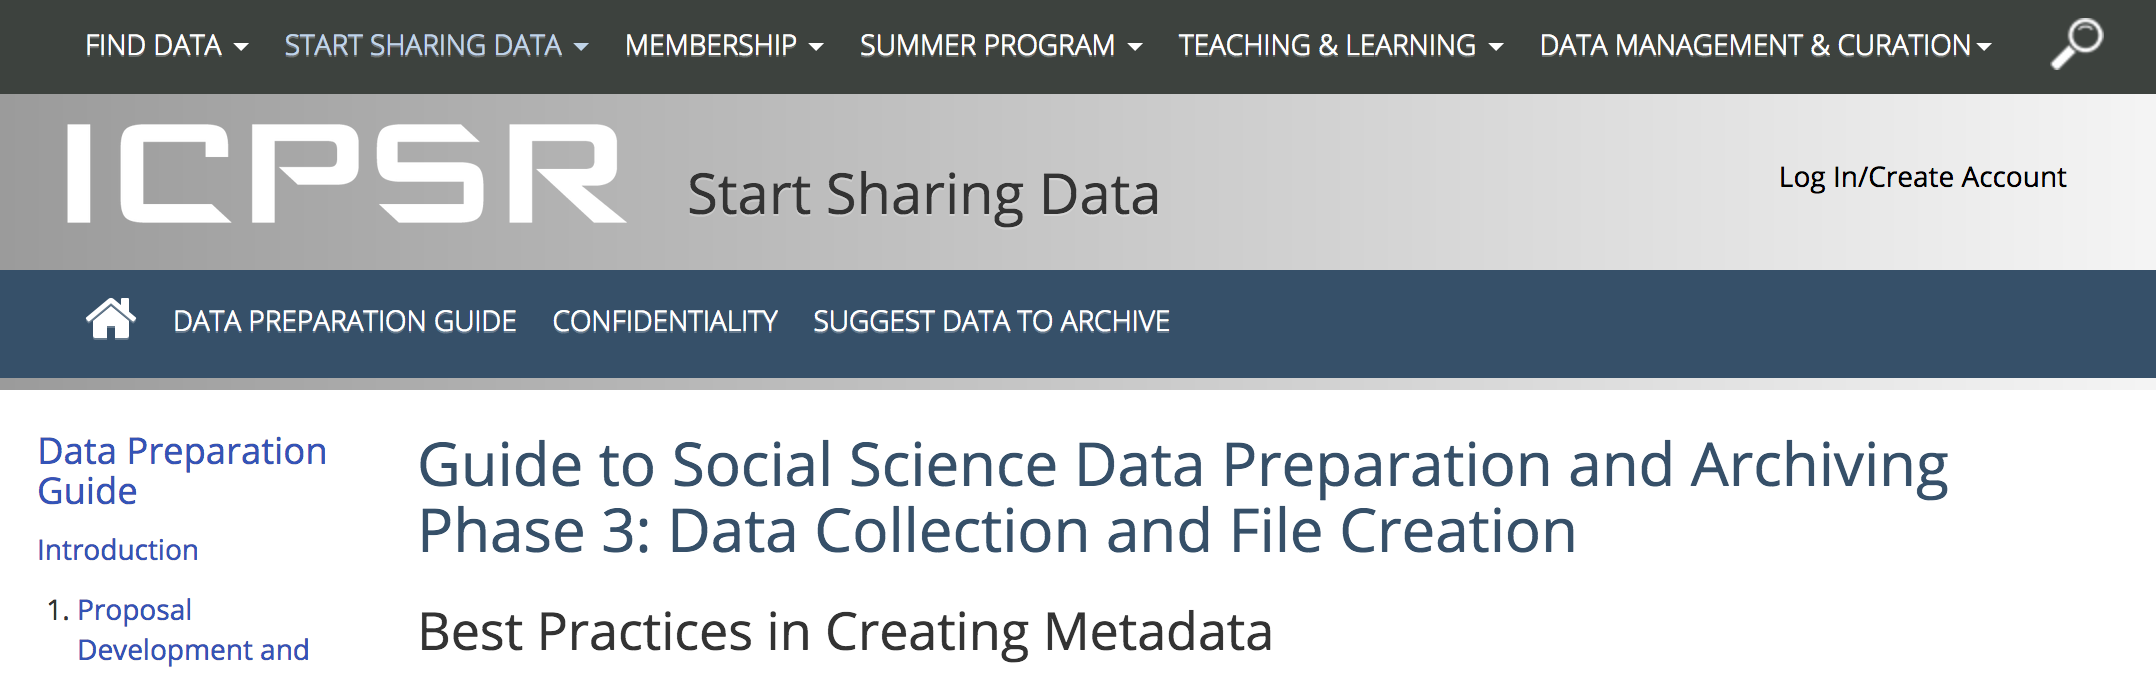
\includegraphics[width=0.9\textwidth]{figures/icpsr_metadata}
\end{figure}

\vfill
\url{https://www.icpsr.umich.edu/icpsrweb/content/deposit/guide/chapter3docs.html}

\end{frame}
%%%%%%%%%%%%%%%%%%%%%%%%
\begin{frame}
\frametitle{Beware of privacy}
\pause

Remove personally identifying information 

\begin{figure}
  \centering
  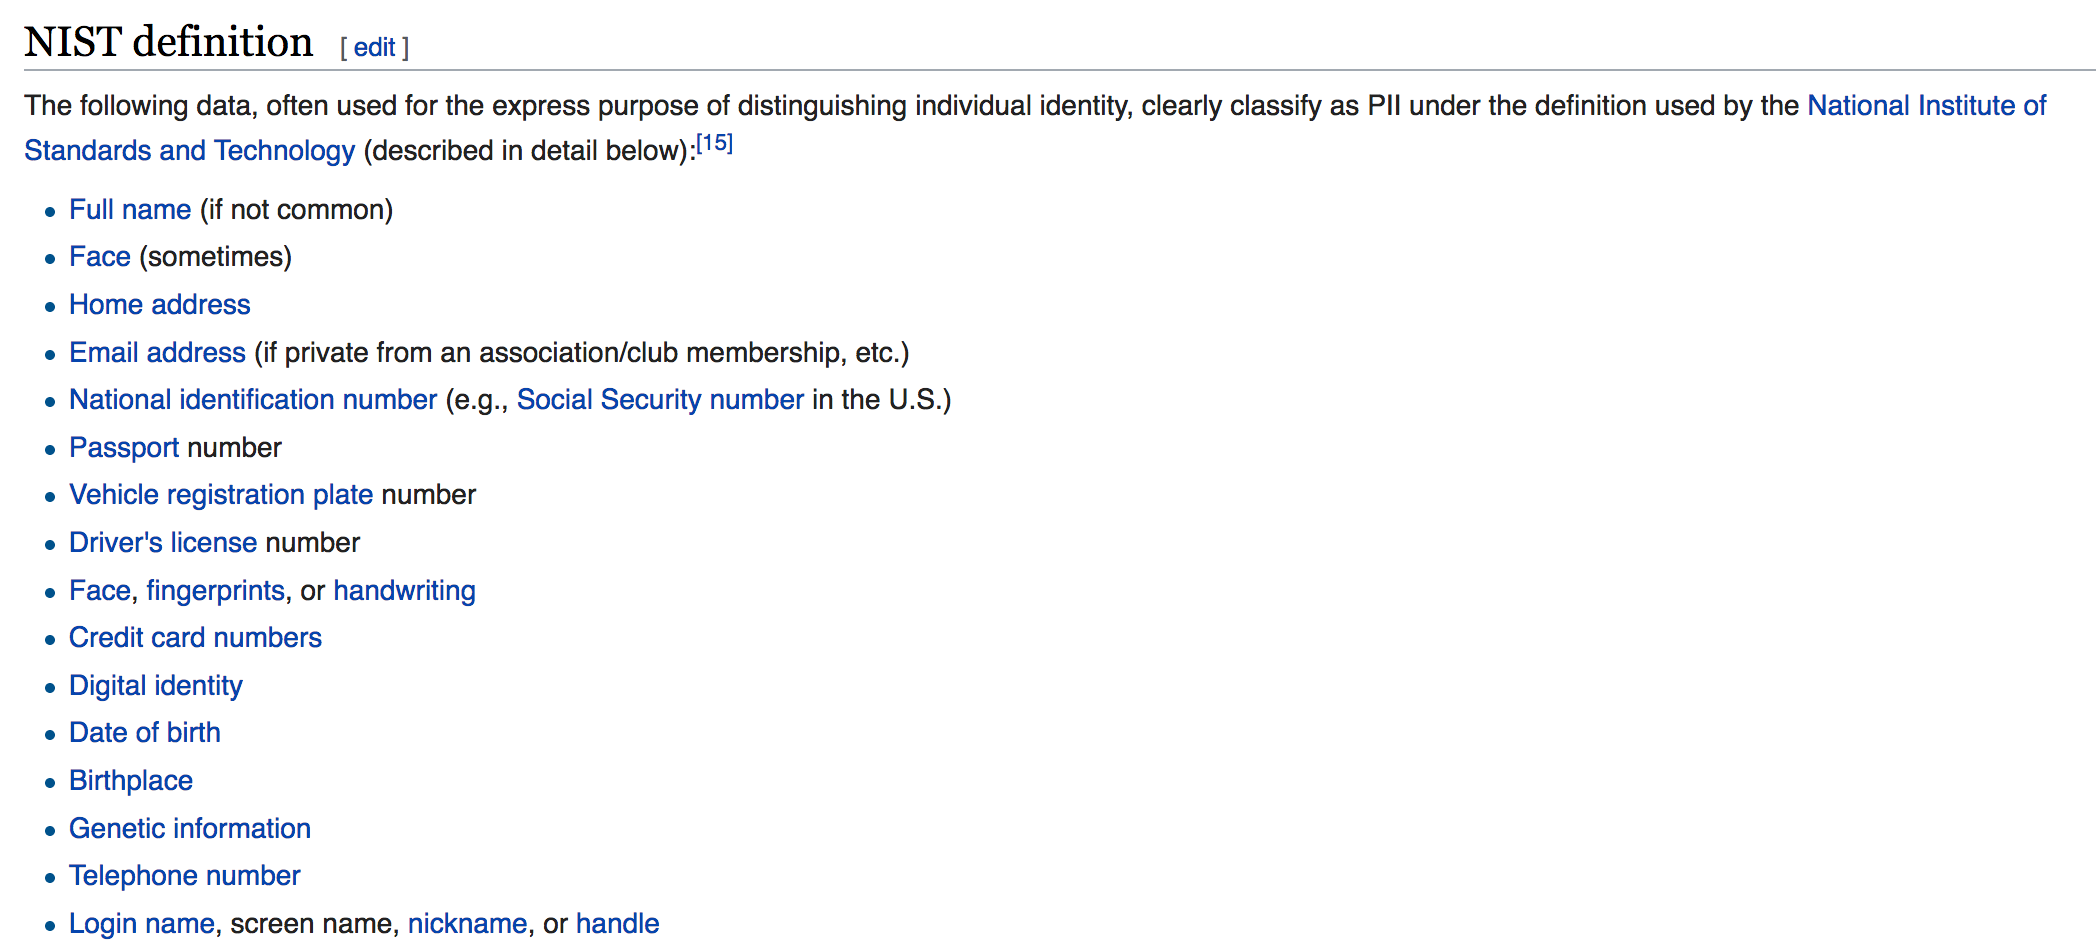
\includegraphics[width=0.9\textwidth]{figures/pii_nist}
\end{figure}

\vfill
\url{https://en.wikipedia.org/wiki/Personally_identifiable_information}

\end{frame}
%%%%%%%%%%%%%%%%%%%%%%%%
\begin{frame}

\begin{figure}
  \centering
  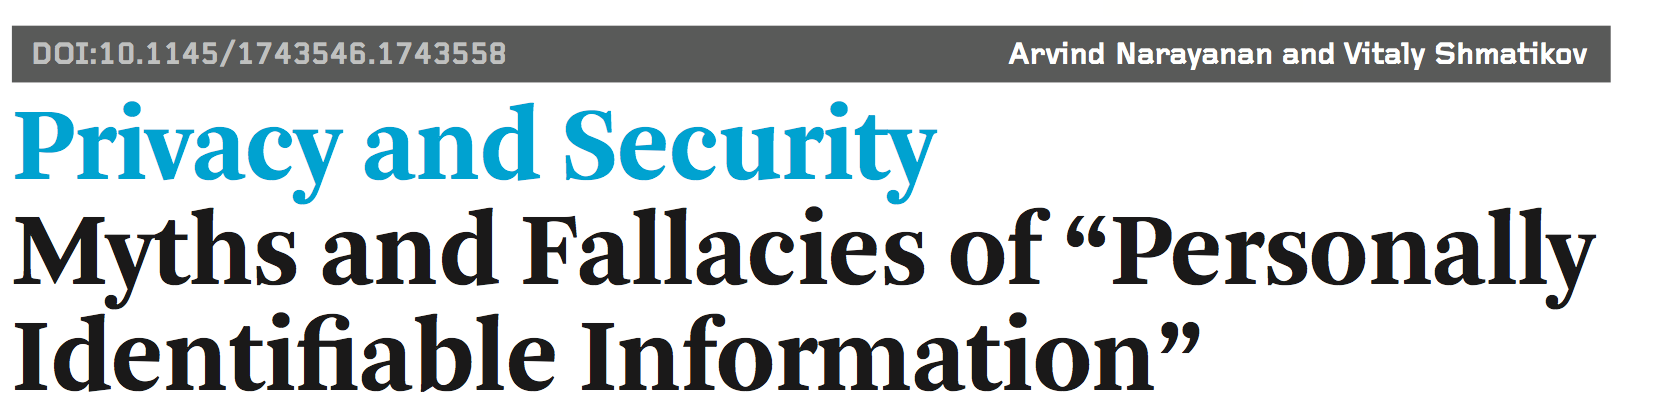
\includegraphics[width=0.9\textwidth]{figures/narayanan_myths_2010_title}
\end{figure}

\vfill
\url{http://dx.doi.org/10.1145/1743546.1743558}
\end{frame}
%%%%%%%%%%%%%%%%%%%%%
\begin{frame}

In this case, we recommend:
\begin{itemize}
\item Removing PII (name, email address, etc)
\item Removing TurkID
\item Coarsen age, geography, and race/ethnicity
\item Coarsen timestamp
\item Anything else?
\end{itemize}

For more on coarsening, see this code: [ link to Janet's data cleaning code ]
\end{frame}
%%%%%%%%%%%%%%%%%%%%%%%%%%
\begin{frame}

For more about de-identification, see \textit{Bit by Bit}, Sec 6.6.2 \href{https://www.bitbybitbook.com/en/1st-ed/ethics/dilemmas/info-risk/}{\textcolor{blue}{``Understanding and managing informational risk''}}

\end{frame}
%%%%%%%%%%%%%%%%%%%%%%%%%%
\begin{frame}

The 5Ws of data release: \pause
\begin{itemize}
\item Who: You
\pause
\item What: make your data available to other researchers in a responsible way
\pause
\item Where: Dataverse, ICPSR, or an archival data repository \pause (your laptop is not an archival data repository)
\pause 
\item When:  when you publish your paper
\pause
\item Why: It is good for you and it is good for the world
\end{itemize}

\end{frame}
%%%%%%%%%%%%%%%%%%%%%%%%%%
\begin{frame}

In this case, you should archive your data here:\\
\url{https://github.com/compsocialscience/summer-institute/tree/master/2018/materials/day4-surveys/datasets}

\end{frame}
%%%%%%%%%%%%%%%%%%%%%%%%%%
\begin{frame}

When you start your projects next week
\begin{itemize}
\item plan to release your data
\item plan to release your code
\end{itemize}

\end{frame}
%%%%%%%%%%%%%%%%%%%%%%%%%%
\begin{frame}

\begin{center}
\LARGE Questions
\end{center}

\end{frame}
%%%%%%%%%%%%%%%%%%%%%%%%%%



\end{document}
